\documentclass[a4paper,11pt]{article}
\usepackage[utf8]{inputenc}
\usepackage{lastpage}
\usepackage{fancyhdr}
\usepackage[english]{babel}
\usepackage[a4paper,margin=1in]{geometry}
\usepackage{multirow}
\usepackage[table,xcdraw]{xcolor}
\usepackage{array}
\usepackage{graphicx}
\usepackage{caption}
\usepackage{ctable}
\usepackage{listings}

\newcolumntype{L}[1]{>{\raggedright\let\newline\\\arraybackslash\hspace{0pt}}m{#1}}
\newcolumntype{C}[1]{>{\centering\let\newline\\\arraybackslash\hspace{0pt}}m{#1}}
\newcolumntype{R}[1]{>{\raggedleft\let\newline\\\arraybackslash\hspace{0pt}}m{#1}}

\newcommand\tab[1][4mm]{\hspace*{#1}}


%-------------------------------------------------------------------------------
% HEADER & FOOTER
%-------------------------------------------------------------------------------

\pagestyle{fancy}
\fancyhf{}
\setlength\headheight{15pt}
\fancyhead[L]{ Imaging Lab 3 }
\fancyhead[R]{Student ID: 100633486}
\fancyfoot[R]{Page \thepage\ of \pageref{LastPage}}


%-------------------------------------------------------------------------------
% TITLE PAGE
%-------------------------------------------------------------------------------

\begin{document}

\title{
	\Huge \textbf {Linear Filters}
    \\ [0.2cm]
	\LARGE Imaging Lab 3 - May, 2017
    \\ [0.5cm]
    \hrule
}

\date{}

\author{
		\Large Kamyar Nazeri \\
		\large Student ID: 100633486 }

\maketitle
\newpage

\section*{Running Cadets}
To make it look like the cadet in the foreground is running faster, we use \emph{Motion Blur} on the region containing the cadet. The length and the angel used in this report are 12 pixels and 10 degree respectively: $fspecial('motion', 12, 10);$
\\\\
To apply the filter on the selective region, we use \emph{roifilt2} command on 3 color channels. However using \emph{roifilt2} creates sharp edges around the foreground cadet. An alternative solution is to first use \emph{imfilter} command on a masked image (foreground cadet region) and then project the filtered image on the original image using Matlab's \emph{image} class. By using this technique, there will be no sharp edges around the foreground cadet. \emph{Figure 1} shows both techniques alongside the original image:

\begin{figure}[!htb]
  \centering
  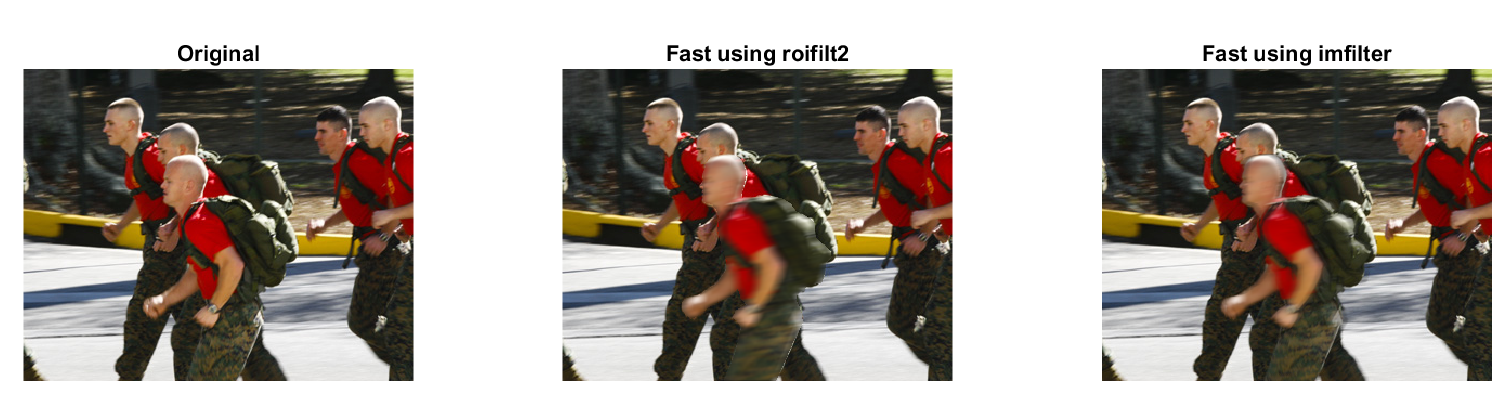
\includegraphics[width=16cm, height=4cm]{1.png}
  \caption{\small Filter the cadet in the foreground to make it look like he is running faster than the others}
\end{figure}

 \\To make it look like the cadet in the foreground is running slower, we can decrease the motion blur by using deconvolution. The length and the angel used in this report are 2 pixels and 40 degree respectively. We can also use \emph{unsharp} mask to sharpen the image in the region of the foreground cadet, and make it appear that the cadet is running slower than the rest of the group. The value of the unsharp mask used in this report is 0.5. \emph{Figure 2} shows both techniques alongside the original image:

\begin{figure}[!htb]
  \centering
  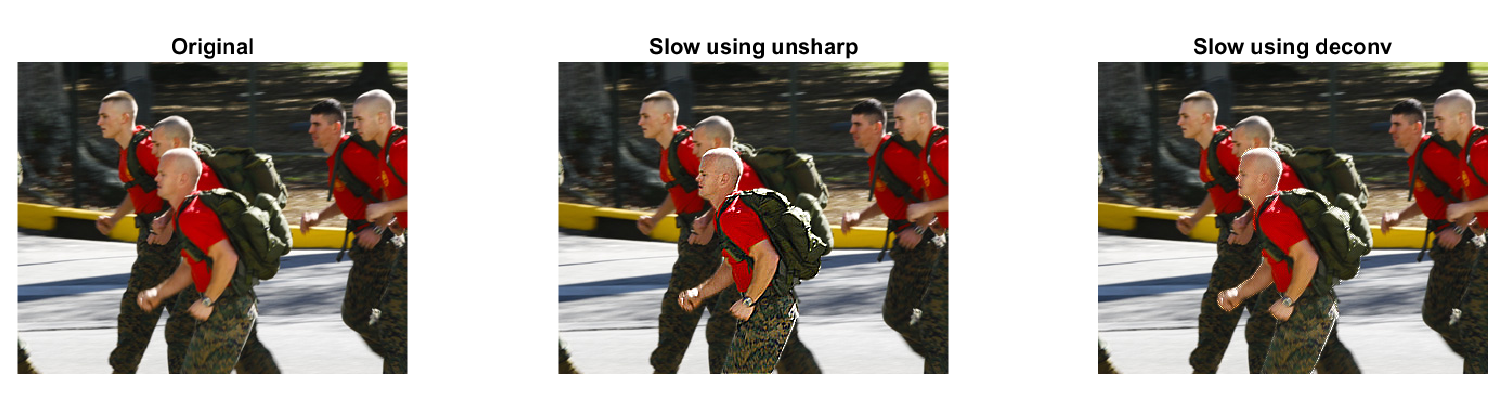
\includegraphics[width=16cm, height=4cm]{2.png}
  \caption{\small Filter the cadet in the foreground to make it look like he is running slower than the others}
\end{figure}

\newpage
\section*{Waterfall}
To make it look like the water is falling faster, we use \emph{Motion Blur} filter on some regions of the image. Because the water is falling in different angels in the image we use 6 different \emph{Motion Blur} filters on 6 regions of the image. The length and the angel used in this report are as follows: \\
region 1: 30 pixel, -80 degree \\
region 2: 30 pixel, -60 degree \\
region 3: 30 pixel, -10 degree \\
region 4: 30 pixel, 5 degree \\
region 5: 30 pixel, 0 degree \\
region 6: 30 pixel, 20 degree \\
\\
To apply the filter on the selective regions, we use \emph{roifilt2} command on 3 color channels. \\
To make it look like the water is falling slower, we use \emph{unsharp} mask to sharpen the image in all 6 regions. The value of the \emph{unsharp mask} used is 0.9 for all regions. To smooth the edges of the waterfall, when applying filters, we use 8x8 \emph{Mean} filter on the regions containing edges. \emph{Figure 3} shows the \emph{Fast} and the \emph{Slow} filters applied on the image alongside the original image:

\begin{figure}[!htb]
  \centering
  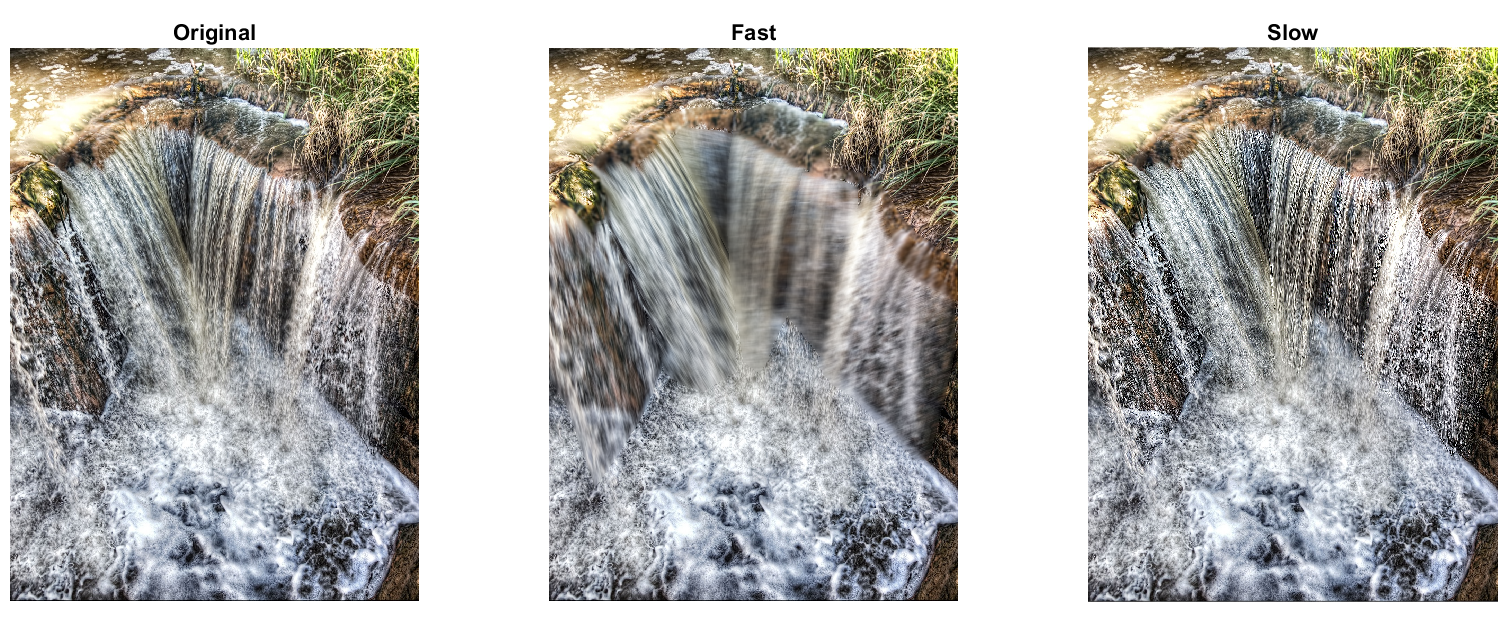
\includegraphics[width=16cm, height=6cm]{3.png}
  \caption{\small Filter the water to makes it look like it is falling faster/slower}
\end{figure}

\newpage

\section*{Rainbow}
To insert a translucent rainbow into the waterfall image, we create a color gradient and a mask and then incorporate the masked image into the waterfall image.\\
\emph{Figure 4} shows the rainbow gradient, the mask and the masked image:
\begin{figure}[!htb]
  \centering
  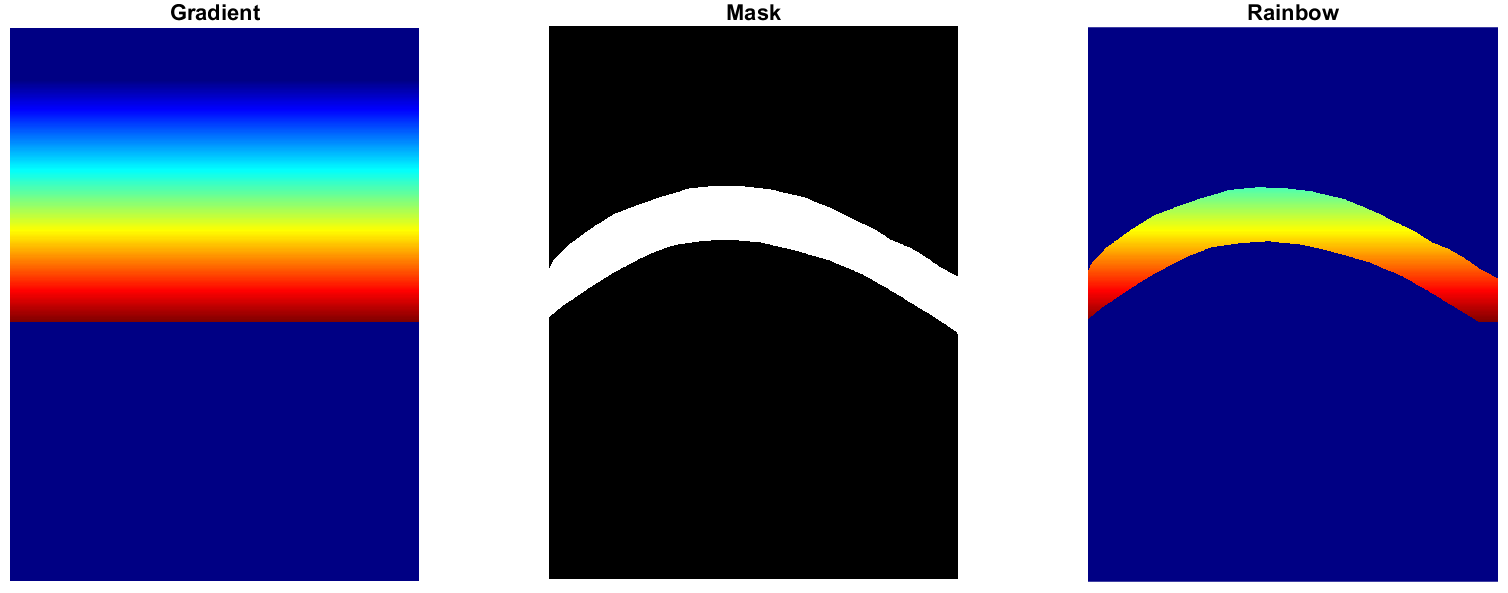
\includegraphics[width=14cm, height=6.6cm]{mask.png}
  \caption{\small Rainbow color gradient and the mask}
\end{figure}

\emph{Figure 5} shows a translucent rainbow added into the waterfall image by manipulating the RGB values in Matlab:
\begin{figure}[!htb]
  \centering
  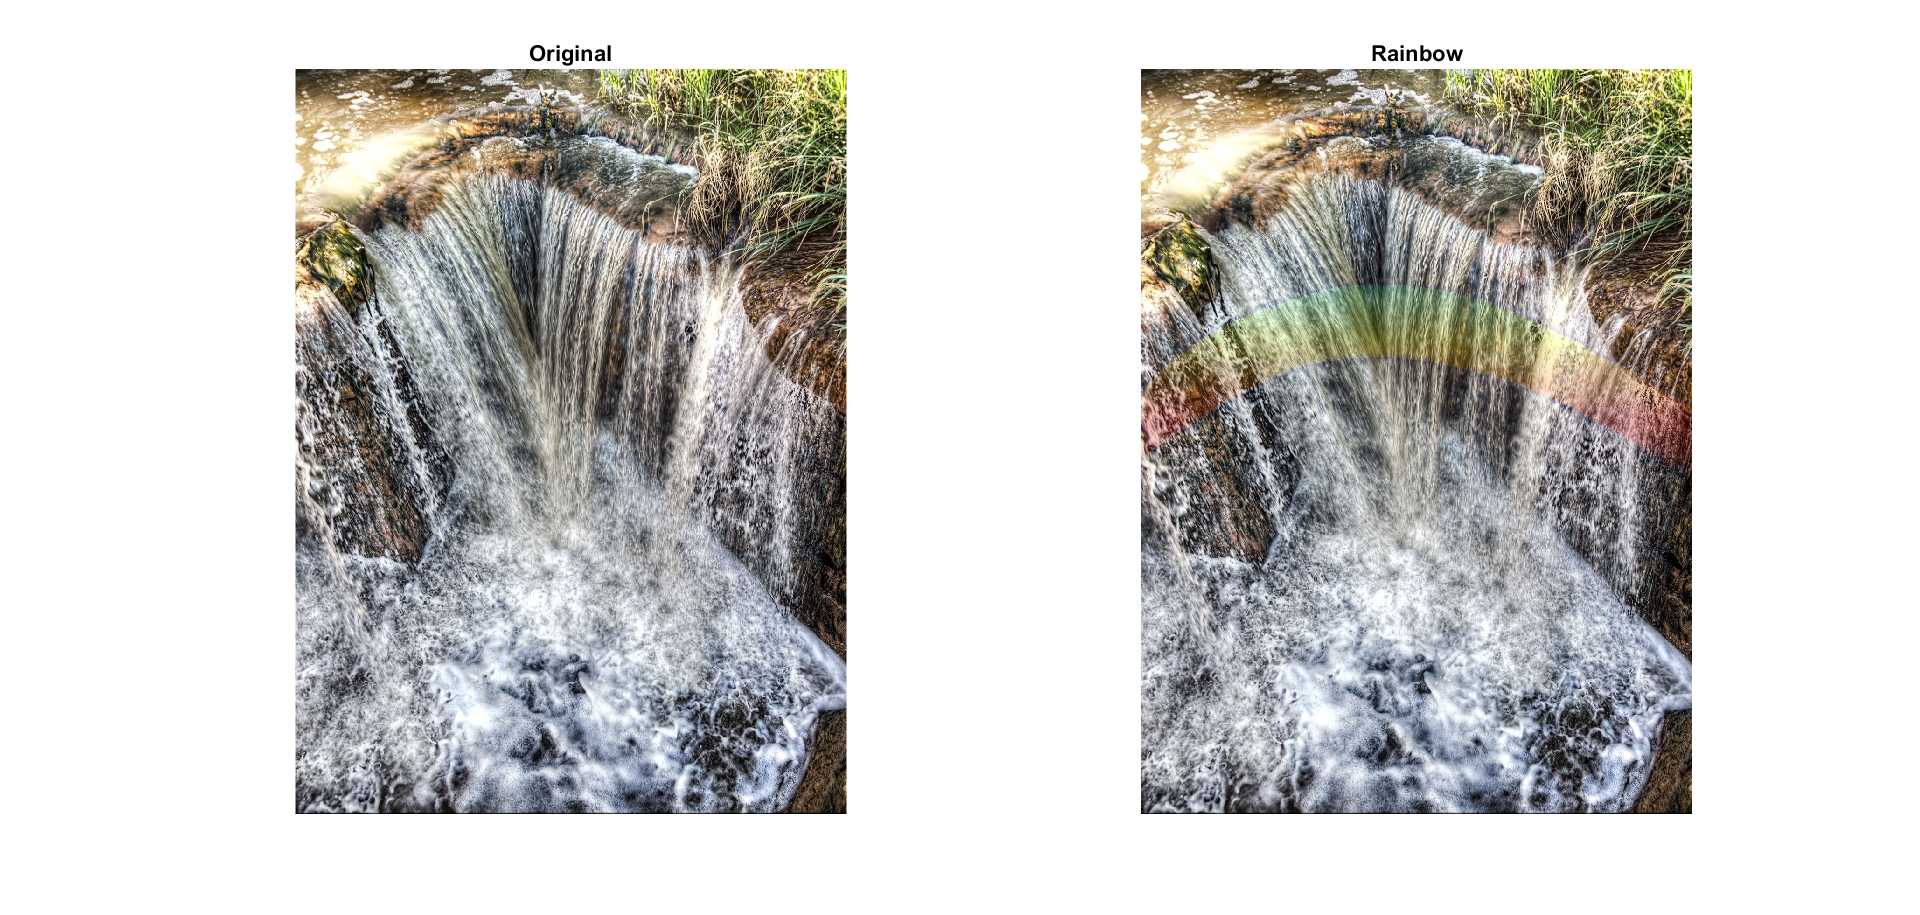
\includegraphics[width=14cm, height=6.6cm]{4.png}
  \caption{\small Translucent rainbow added into the waterfall image}
\end{figure}

\end{document}
